\chapter{Metodología y desarrollo}

Este capítulo describe el flujo de trabajo propuesto para usar \textit{HDL Coder} y \textit{HDL Verifier}, los casos de estudio seleccionados y la metodología de validación en simulación y \textit{FIL}. El contenido complementa el material disponible en el repositorio de código, que concentra scripts, modelos y bitstreams necesarios para reproducir y extender los resultados.

\section{Flujo de trabajo}

El flujo considera: ajuste del modelo en Matlab/Simulink para tipos y estructuras sintetizables; configuración de \textit{HDL Coder} para generación RTL; co-simulación y \textit{FIL} con \textit{HDL Verifier} para equivalencia funcional; y registro de configuraciones y reportes en el repositorio. Cada caso de estudio sigue la misma secuencia para facilitar la comparación entre algoritmos.

En términos operativos, la secuencia se implementa en seis pasos:
\begin{enumerate}
    \item \textbf{Definición del DUT y banco de pruebas}: se selecciona el bloque o función objetivo y se construye un \textit{testbench} reproducible, con entradas representativas y criterio de comparación explícito.
    \item \textbf{Conversión y validación numérica}: cuando el diseño parte en flotante, se propone tipo fijo, se ajustan fracciones y se valida el error respecto al modelo de referencia.
    \item \textbf{Generación HDL y análisis de reportes}: se ejecuta el \textit{Workflow Advisor}, revisando latencia, requerimientos de reloj interno y reportes de recursos para decidir ajustes de optimización.
    \item \textbf{Análisis de resultados de recursos, ciclos internos y ciclos de latencia}: se consolidan métricas de síntesis para comparar variantes de arquitectura y verificar coherencia entre costo de hardware y desempeño temporal.
    \item \textbf{Verificación en co-simulación y FIL}: se contrasta la salida HDL frente al modelo original y se comprueba comportamiento temporal bajo la configuración de \textit{overclocking}/\textit{oversampling} correspondiente.
    \item \textbf{Trazabilidad y empaquetado}: se registran configuraciones, bitstreams, scripts y resultados para permitir repetición del experimento o extensión a variantes del caso.
\end{enumerate}

Este esquema se repite en todos los ejemplos porque permite comparar resultados con el mismo criterio metodológico y, al mismo tiempo, aislar con mayor claridad qué efecto produce cada decisión de modelado o síntesis.

Como criterio de control de calidad, cada iteración del flujo se cerró con una revisión mínima de cuatro puntos: integridad del testbench, coherencia de tipos en interfaces, consistencia temporal (latencia y sobre-reloj) y reporte de recursos. Si uno de estos puntos fallaba, la iteración no se consideraba válida para comparación en el capítulo de resultados. Esta regla simple evitó acumular variantes no comparables y mejoró la trazabilidad del proceso.

\begin{figure}[tbp]
    \centering
    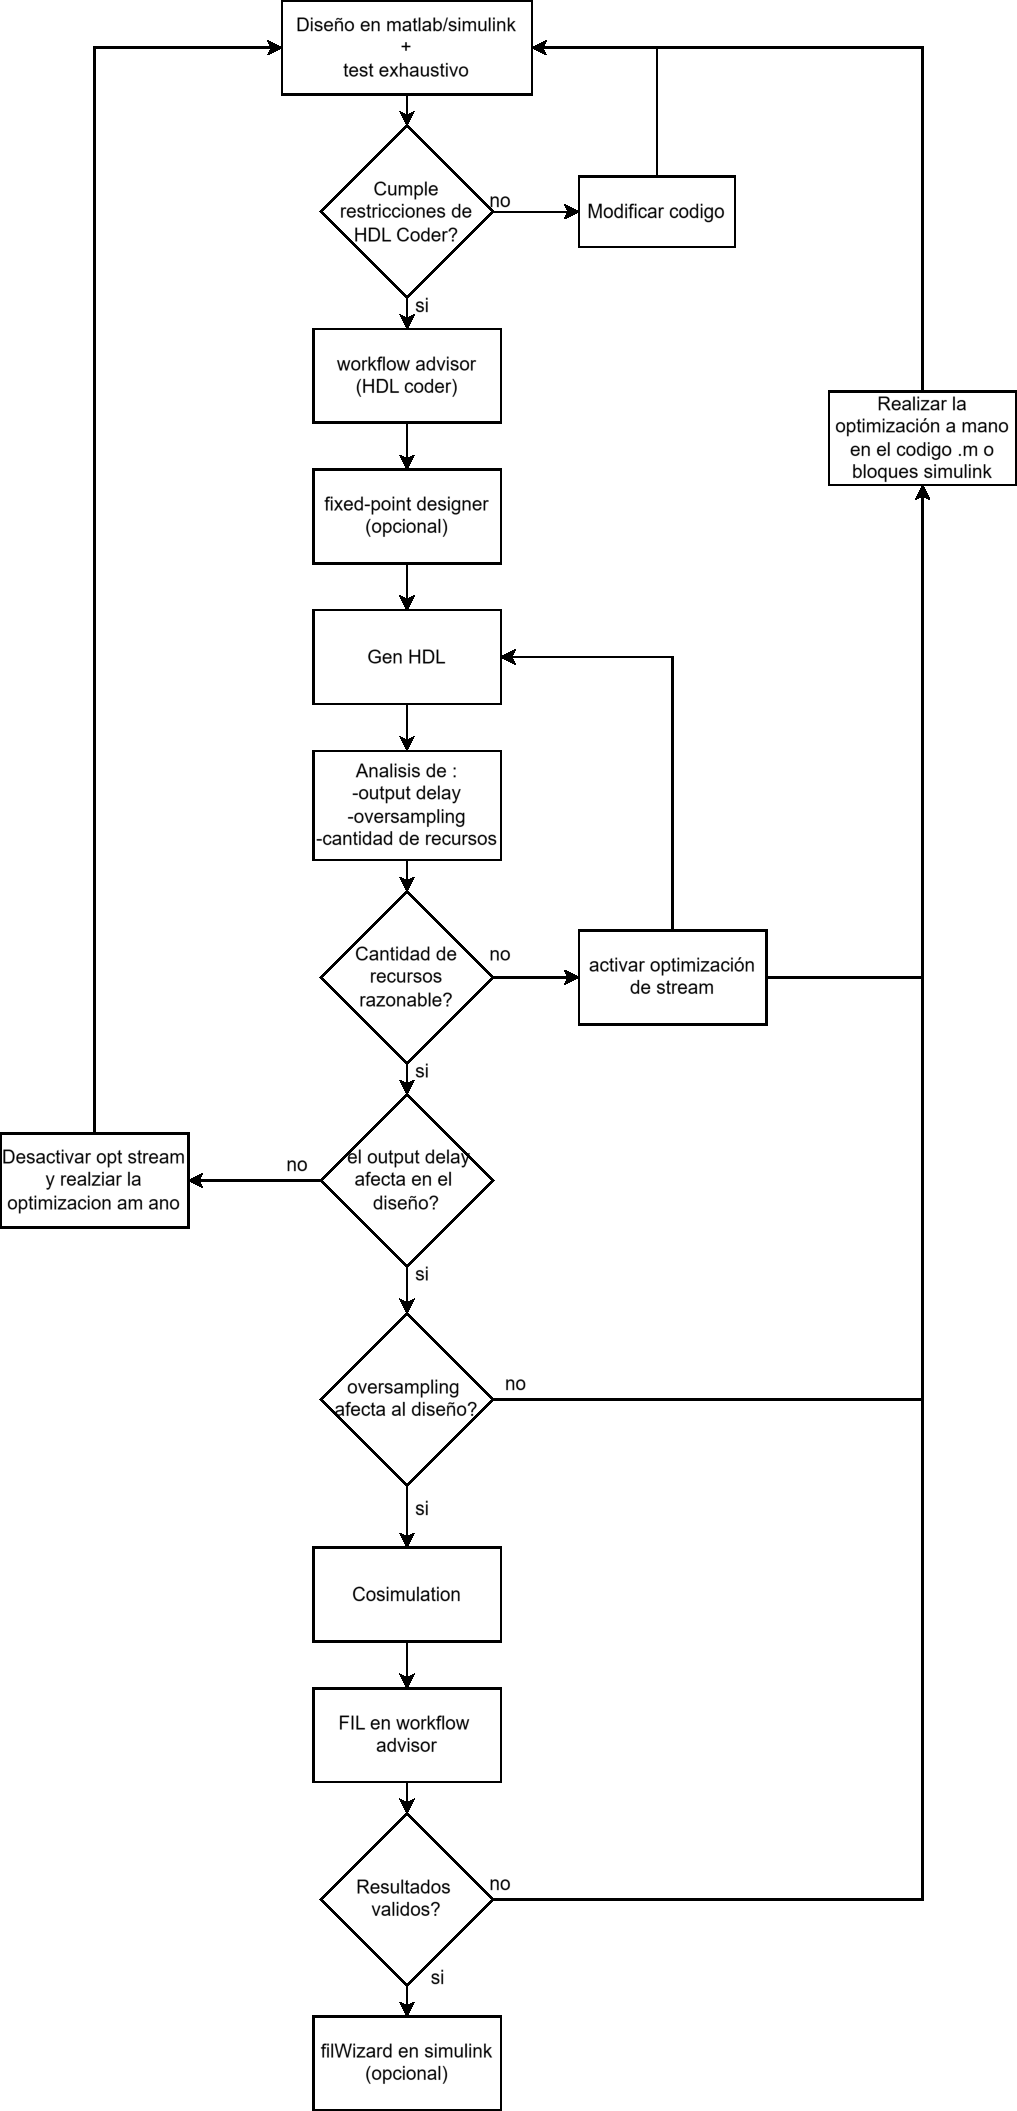
\includegraphics[width=0.62\textwidth,height=0.80\textheight,keepaspectratio]{fig/Diagram_V4.pdf}
    \caption{Flujo de buenas prácticas para usar HDL Coder en la generación y validación de HDL.}
    \label{fig:flujo_hdl_coder_buenas_practicas}
\end{figure}


\section{Aplicaciones de ejemplo}

Los ejemplos seleccionados cubren control, verificación y cómputo intensivo para validar el flujo completo sin entrar en el detalle de cada implementación. Se incluyen: producto punto (flujo base y comparación fixed vs floating), PID con anti-windup (lazo cerrado y \textit{FIL}), controlador PI para estudiar \textit{overclocking}, contador para caracterizar muestreo, MPC/ADMM como caso exigente en recursos, y un núcleo de SNN para evaluar procesamiento por eventos. El objetivo de esta selección es obtener conclusiones comparables sobre equivalencia funcional, latencia y uso de recursos en distintos perfiles de diseño.

La selección no fue arbitraria: se buscó cubrir patrones de diseño complementarios. Producto punto representa un caso de datapath acotado, útil para observar de forma controlada el efecto de cuantización y compartición de operadores. PID y PI representan sistemas con realimentación, sensibles a retardo y saturación. El contador aporta una referencia temporal simple para estimar sobre-reloj requerido. SNN incorpora alto fan-in y empaquetado de señales, mientras ADMM/MPC tensiona el flujo en complejidad algorítmica y costo de recursos.

Con este conjunto, el flujo se evalúa en dimensiones distintas pero comparables: fidelidad funcional, robustez temporal y viabilidad de implementación. En otras palabras, cada ejemplo cumple un rol metodológico dentro del análisis global y no solo una función demostrativa aislada.

\subsection{Producto punto}

El caso de producto punto se utiliza como referencia base del flujo porque permite controlar con claridad la relación entre precisión numérica, latencia y utilización de recursos. El proceso parte con una función MATLAB simple y un banco de pruebas con múltiples entradas aleatorias para construir una referencia ``golden''. A partir de esa referencia se ejecuta la conversión a punto fijo y la validación numérica, de modo que el diseño HDL se genere desde tipos y rangos coherentes con los datos de prueba.

En la etapa de generación se evaluaron dos configuraciones: con y sin \textit{stream loops}. Con \textit{stream loops}, el compilador comparte operadores aritméticos y exige un reloj interno más rápido, reduciendo recursos a costa de aumentar las restricciones temporales. Sin \textit{stream loops}, el diseño queda más directo y combinacional, con menor complejidad de control pero peor escalabilidad cuando el tamaño del problema aumenta. El ejemplo también se ejecutó en punto flotante para contrastar costo en hardware frente a punto fijo, observándose un crecimiento importante de recursos para una mejora numérica que en este caso no era crítica.

Este caso también se utilizó para validar la disciplina de pruebas que luego se aplicó al resto de ejemplos: almacenamiento de señales de referencia, repetición de estímulos entre corridas y comparación explícita de salida esperada vs salida HDL. Al mantener fijo el conjunto de pruebas entre variantes, fue posible atribuir diferencias a cambios de arquitectura y no a cambios de estímulo.

\subsection{PID con anti-windup}

El ejemplo de PID con anti-windup se orienta a validar un flujo de control en lazo cerrado con parámetros configurables desde Simulink. El controlador se modela en tiempo discreto incorporando saturación de actuador y realimentación anti-windup en el integrador. Para la etapa HDL se fijan tipos \textit{fixed-point} en entradas y bloques aritméticos, con saturación explícita en \textit{overflow}, lo que reduce discrepancias entre el modelo de alto nivel y el comportamiento del HDL generado.

La verificación se realiza en dos niveles: primero por co-simulación y luego por \textit{FPGA-in-the-Loop}. En ambas etapas se comparan señales del lazo cerrado para distintos escenarios de referencia y distintos valores de ganancia anti-windup. Esta secuencia permite observar, sobre un caso de control realista, cómo la elección de tipos y escalamiento impacta tanto la calidad de respuesta como la reproducibilidad funcional entre simulación y hardware.

En términos de implementación, este ejemplo fue clave para fijar lineamientos sobre señales de frontera entre dominios discretos y continuos. El uso de bloques de retención de orden cero y conversiones de tipo en puntos bien definidos evitó inconsistencias de muestreo y mejoró la interpretabilidad de resultados. Además, permitió analizar el efecto práctico de modificar parámetros del controlador sin regenerar por completo el entorno de validación.

\subsection{PI y contador para análisis de muestreo}

Los ejemplos de PI y contador se usan como casos instrumentales para estudiar el \textit{overclocking factor}. En el PI, el comportamiento esperado se recupera cuando el \textit{overclocking} coincide con los ciclos internos requeridos por el diseño; valores menores generan submuestreo y valores muy altos alteran la dinámica de la respuesta. En el contador, el efecto es aún más explícito: cada salida interna tiene una frecuencia distinta, por lo que el valor observado en Simulink depende de cuántos ciclos de FPGA se acumulan por cada muestra externa.

Ambos ejemplos se incluyeron porque entregan una regla práctica para configurar \textit{FIL}: no basta con que el diseño sintetice, también debe existir coherencia entre la temporalidad interna del HDL y la temporalidad del banco de pruebas. Esta consideración se aplica luego al resto de casos, en particular a arquitecturas con latencia multicíclo.

Desde el punto de vista metodológico, PI y contador funcionaron como ``instrumentos de calibración'' del flujo. Antes de validar casos más complejos, estos ejemplos permitieron comprobar que la infraestructura de pruebas (conexión FIL, sincronización y observación de señales) respondía de manera consistente frente a cambios controlados de \textit{overclocking}. Esta calibración previa redujo incertidumbre al interpretar resultados de SNN y ADMM.

\subsection{SNN con y sin \textit{stream}}

El núcleo SNN incorpora un patrón de cómputo por eventos y un ancho de entrada alto (784 señales binarias), lo que obliga a definir una estrategia de interfaz adecuada para \textit{FIL}. En lugar de exponer cientos de puertos escalares, las entradas se empaquetan en un bus \texttt{ufix784}, permitiendo ejecutar pruebas por tramas sin perder trazabilidad con el modelo de referencia.

Para este caso se compararon dos variantes de síntesis: con \textit{stream} y sin \textit{stream}. La versión con \textit{stream} prioriza compartición de recursos y mantiene un costo de hardware acotado; la versión sin \textit{stream} favorece paralelismo estructural y aumenta de forma marcada el número de operadores. Esta comparación se incorporó para mostrar que, en diseños de gran fan-in, la política de compartición no es un ajuste secundario, sino una decisión de arquitectura que condiciona la factibilidad de implementación.

Adicionalmente, SNN permitió validar una estrategia de empaquetado de datos reutilizable en otros diseños con gran número de entradas binarias. Al transportar la información como bus compacto y mantener una convención consistente de orden de bits, se simplificó la integración con \textit{FIL} y se redujo la complejidad de cableado del modelo de prueba.

\subsection{ADMM/MPC como caso de estrés}

El ejemplo ADMM/MPC representa el caso de mayor exigencia del conjunto. El algoritmo original, sin modificaciones para hardware, tiende a producir un RTL muy costoso en operadores y difícil de cerrar temporalmente. Por ello, el flujo incluye una fase previa de adecuación: acotar iteraciones, reordenar operaciones matriciales y privilegiar estructuras que faciliten \textit{resource sharing}.

Este caso cumple dos funciones dentro de la metodología: validar que el flujo también opera sobre algoritmos de optimización más complejos y, al mismo tiempo, establecer límites prácticos del enfoque automático. En términos de documentación, ADMM/MPC actúa como referencia para discutir los compromisos entre precisión, latencia y recursos cuando se escala a aplicaciones de mayor complejidad.

La experiencia con ADMM/MPC también reforzó un criterio transversal de esta memoria: cuando un diseño no converge a una implementación razonable, la solución no suele ser ``forzar más opciones'' de la herramienta, sino rediseñar el cómputo para adaptarlo al modelo de hardware. Esta conclusión, aunque conocida en teoría, adquiere valor práctico al observarse de forma repetida en un caso real de alta exigencia.

\section{Plataformas objetivo y configuraciones}

Se emplean FPGAs de distintas gamas para validar funcionalidad y latencias: placas con dispositivos Artix/Cyclone para perfiles de recursos acotados y SoC reconfigurables (por ejemplo, Zynq) para evaluar integración con procesadores embebidos. Para \textit{FIL} se definen relojes, interfaces de E/S y restricciones mínimas necesarias para ejecutar los bancos de pruebas sin optimizaciones específicas de plataforma.

La política de configuración priorizó portabilidad sobre ajuste fino. Es decir, se evitó sobre-optimizar cada caso para una única tarjeta y se privilegió una configuración estable que pudiera repetirse entre variantes. Esta decisión reduce el desempeño máximo alcanzable en algunos ejemplos, pero aumenta la comparabilidad de resultados y la utilidad del flujo como guía de trabajo general.

\section{Implementaciones}

Cada implementación incluye scripts de generación, archivos de proyecto y bancos de prueba. Los casos de control (PID y MPC) se verifican contra modelos de planta en \textit{Simulink}, midiendo error de seguimiento y comportamiento bajo saturación. El núcleo SNN se valida con patrones de disparo conocidos y monitoreo de eventos para asegurar coincidencia con el modelo de referencia. Reportes de uso de recursos y frecuencia estimada se almacenan junto a los bitstreams generados.

Además, se mantuvo una convención común para documentar resultados: en cada ejemplo se reportan (i) configuración de tipos y optimizaciones, (ii) latencia observada o esperada, (iii) recursos principales de síntesis y (iv) comentario de equivalencia funcional en co-simulación/FIL. Esta forma de registro permite que el capítulo de resultados compare casos heterogéneos sin perder consistencia de lectura.

En la práctica, esta convención también permitió construir una línea de base para futuras extensiones. Cualquier nuevo caso que siga la misma estructura de documentación puede incorporarse al repositorio y compararse con los existentes sin redefinir métricas ni cambiar el formato de reporte. De esta manera, la memoria no solo describe un conjunto de experimentos, sino que deja establecido un método de trabajo escalable.
